\chapter{Odpowiedzi skokowe}
\label{zad2}

\section{Wyznaczanie odpowiedzi skokwych}
\label{zad2_skoki}

\begin{figure}[t]
\centering
    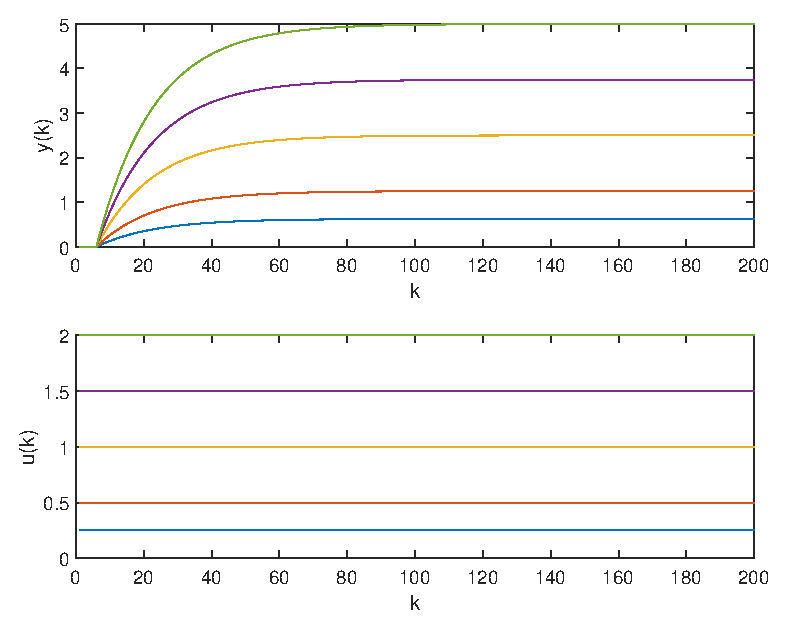
\includegraphics[scale=1]{Rys/odp_skok_u.eps}
    \caption{Odpowiedz procesu na skokową zmiane sterowania}
    \label{zad2_odp_skok_u}
\end{figure}

\begin{figure}[t]
	\centering
	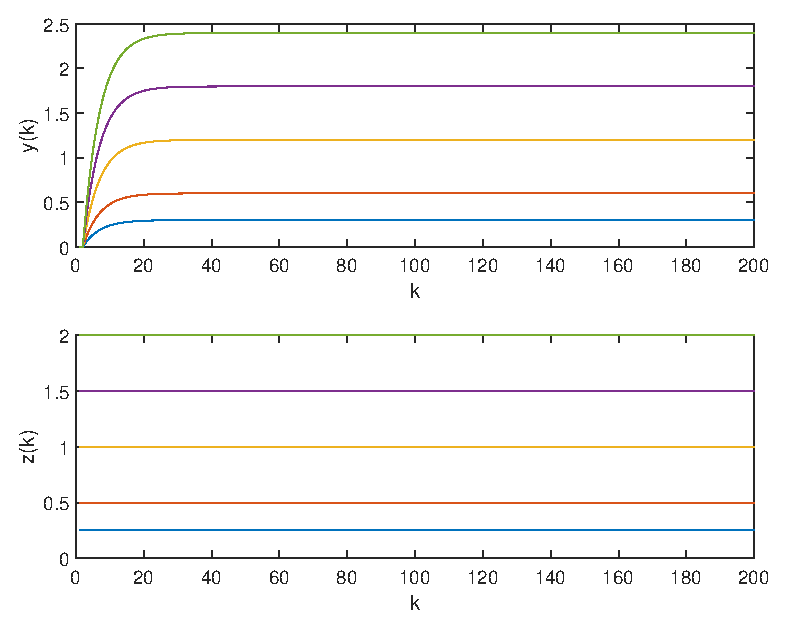
\includegraphics[scale=1]{Rys/odp_skok_z.eps}
	\caption{Odpowiedz procesu na skokową zmiane zakłócenia}
	\label{zad2_odp_skok_z}
\end{figure}

W celu wyznaczenia odpowiedzi skokowej obiekt, znajdujący się w punkcie pracy (tzn. $u= \num{0.0}$, $z= \num{0.0}$, $y= \num{0.0}$) pobudzony zostaje skokową wartością sterowania/zakłócenia. Rysunek \ref{zad2_odp_skok_u} oraz \ref{zad2_odp_skok_z} przedstawia odpowiedź obiektu na dane skoki.

\section{Wyznaczanie charakterystyki statycznej procesu}
\label{zad2_char_stat}
Aby wyznaczyć charakterystykę statyczną procesu przeprowadzono analogiczne działania co w rozdziale \ref{zad1}. Tym razem przy użyciu skryptu \verb+Zad2.m +dla wielu wartosci $u$ oraz $z$ wyznaczono odpowiadające im $y$ oraz z ich pomocą utworzono wykres \ref{zad2_char_stat}. Jak widać charakterystyka statyczna obiektu jest liniowa, a co za tym idzie obiekt jest liniowy.

\begin{figure}[b]   
     \label{zad2_char_stat}
    \centering
    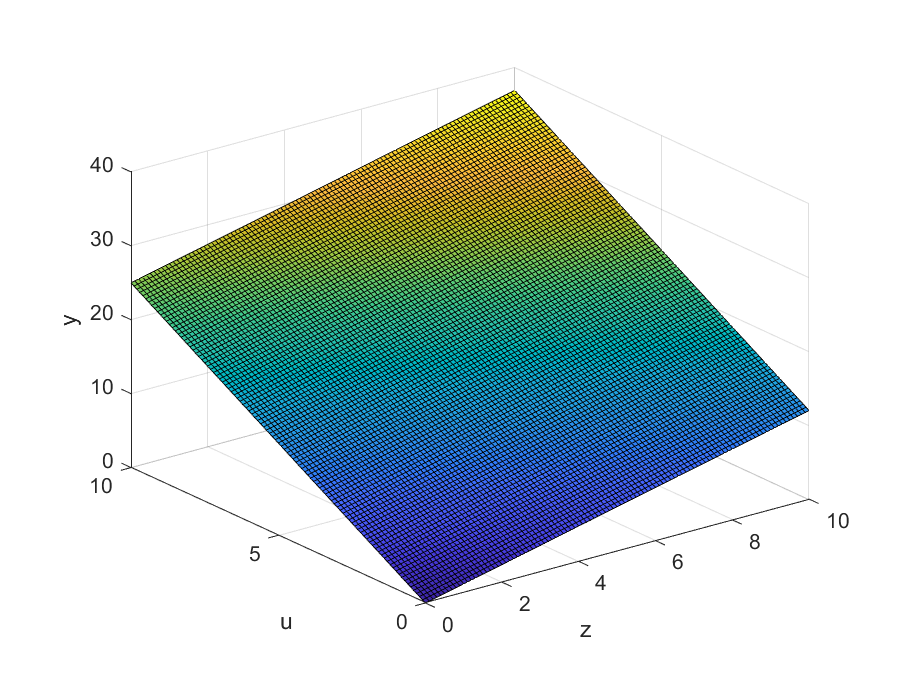
\includegraphics[scale=1]{Rys/char_stat.eps}
    \caption{Charakterystka statyczna $y(u,z)$ symulowanego procesu}

\end{figure}

\section{Wzmocnienie statyczne}
\label{zad2_wzmocnienie}
Wzmocnienie statyczne, czyli stosunek pomiędzy zmianą wartosci wyjscia i zmianą wartosci wejścia w stanie ustalonym. Aby ją wyznaczyć można na przykład znaleźć nachylenie charakterystyki statycznej do osi OU lub OZ, czyli np.:

\begin{equation}
K_{\mathrm{stat}_u} = \frac{y(u_{\mathrm{max}})- y(u_{\mathrm{min}})}{u_{\mathrm{max}}- u_{\mathrm{min}}}
\label{zad2_wzm_statyczne_wzor}
\end{equation}

W przypadku tak wykreślonej charakterystyki, wzmocnienie statyczne jest równe tangensowi kąta $\alpha$
pomiędzy prostą a osią $OU$. 
\begin{equation}
K_{\mathrm{stat}_u} = \frac{24.9903- 0}{10- 0}\approx 2.5
\label{zad2_wzm_statyczne_u}
\end{equation}
\begin{equation}
K_{\mathrm{stat}_z} = \frac{11.9884- 0}{10- 0}\approx 1.2
\label{zad2_wzm_statyczne_z}
\end{equation}
